\documentclass[11pt]{article}
% \usepackage[usenames,dvipsnames,svgnames]{xcolor}

\usepackage{deauthor}
\usepackage{times, enumerate}
\usepackage{graphicx}
\usepackage{authblk}
\usepackage{hyperref,subfigure}
\usepackage{wrapfig}
\usepackage{enumitem}



\begin{document}

\title{Contact Tracing: Holistic Solution Beyond Bluetooth}
%
\author{Ramesh Raskar, Deepti Pahwa, Robson Beaudry \\
{\small \texttt{raskar@media.mit.edu}}\\
MIT Media Labs
}

% \affil{{\small \texttt{\{sseb,biessman,tjnsch,dsalina,seufert,szarvasg
% \}@amazon.com}}}
% \affil{Amazon Research}

\maketitle

\begin{abstract}
Contact tracing is a critical part of reopening society. While manual contact tracing by medical professionals is essential, there’s growing acknowledgement that supplementing this with digital approaches might make a significant difference in the speed with which we can reopen.
 
Safe Paths is open source, standards-based, privacy-first framework that works closely with public health entities. Our approach is to roll out apps, SDKs, privacy-preserving network backbones, and interoperable protocols, so that any developer can build experiences that perform contact-tracing and related activities in safe, easy to use ways.

In this paper, we’ll compare some of the existing technologies that can be used to aid contact tracing and exposure notification efforts, and make the case for using a holistic, multi-modal approach rather than relying exclusively on a single technology.
\end{abstract}

\section{Bluetooth Tracing}

The technology that’s being most widely explored for exposure notification today is Bluetooth Low Energy transmission (BLE); it’s present on most modern mobile devices, and can provide evidence that two phones were near each other. Several groups, including PACT, TCN, BlueTrace, D3PT, and others, have been working together in recent weeks to create privacy-preserving protocols that use Bluetooth for COVID exposure notification. Most recently, Google and Apple have collaborated on a framework for contact tracing apps, which will be extremely helpful in overcoming major barriers to adoption (including interoperability between the two companies’ phones, improvements in battery life, and allowing the use of BLE in the background). (For the rest of this essay, we’ll refer to this Google / Apple Exposure Notification protocol as “GAEN”.) By building contact-tracing support into their operating systems, GEAN could make a difference in adoption of these technologies.

At the same time, there are a host of reasons why the GAEN protocol is not, on its own, a complete solution for contact tracing. Successful contact tracing requires a strong understanding of the context of encounters: where and when did an encounter happen, and what are the chances that the encounter resulted in a transmission? Bluetooth technology does a good job of detecting physical proximity, but it does not provide any other context of the encounters. 

Furthermore, contact tracing (with or without proximity detection) is itself just one piece of the puzzle; public health officials need to be able to generate heatmaps, spread analysis, and other data that allow them to fight this disease holistically. With an understanding of location and context, we can develop that more holistic solution. We need to carefully consider the role of various technologies, their context to the end-user, as well as to the health officials and communities, which we will explore throughout this document.




\paragraph{User experience and App Perspective: The need for a holistic solution with GPS, WiFi and Bluetooth}
There are several reasons to consider a holistic multimodal solution that includes location tracking in addition to  Bluetooth proximity ID. Any one technology has limitations of either false positives, or false negatives. Ultimately, the best solutions will leverage the advantages of GPS, Bluetooth, and WiFi in order to create more accurate, useful, and private data.

\paragraph{Adoption Rate vs Effectiveness:} Bluetooth requires many people to use the apps for it to be valuable. In Singapore the Bluetooth App penetration is 12\% which means only 1.44\% of encounters are recorded (0.12*0.12). As a reference, Casey Newton~\cite{caseynewton} has a good piece on Why Bluetooth apps are bad at discovering new cases of COVID-19. While adoption can be increased through government and big tech buy-in, these numbers still hamper effectiveness.

\paragraph{GPS based App scales linearly:} With a 12\% adoption rate of the app, considering a proportional approach, we might get much better than 12\% coverage in any given area. This means that if 12\% of people install the app. (I.e. if 100 infected people went to the store in a week, and we only caught 12 of them, that's still potentially enough to label it as a hotspot.12\% of infected hotspots will be identified This identification would be very helpful, as nearly everyone in town will hear about them, eg. local news channels. GPS  is useful even if smartphone penetration in a region is not widespread.


\paragraph{False positives or False Negatives:} Attempting to do exposure alerting as the only intervention in such cases has the risk of generating either false positives, or false negatives. For instance, if you are  living in the apartment below an infected person, sharing a ceiling/floor, or working from a neighboring office, such a notification can still flag you as at risk. False negatives could occur if your phone was turned off or not with you when you came into contact with an infected person. This ambiguity can only be handled by a good UX.



\paragraph{Contextual information is key:} Users do not like to get an alert without understanding the context. They need to know where exactly the encounter took place in order to trust the system. This location information can be provided by GPS location logging. Note that adding location and time to BLE encounters make them less private, because in some cases it will allow the person receiving the alert to deduce from whom the alert was sent (if they know they were only in the presence of one other person at the time, for example). But without this contextual information, it’s impossible for the exposed individual to judge the reliability of the notification.

Further, in the context of manual contact tracing by medical professionals, access to location information can help them conduct interviews by helping the patients, for example, remember if they were wearing a mask or not, whether they shook hands or not, etc.


\section{Health Organisations Perspective: Public health needs more than just encounters}


The prime need of the health officials is their ability to \emph{call the exposed person directly to assess their personal situation} and provide guidance about testing/isolation/hospitalization. Health care officials also need \emph{dashboards of emerging hotspots} to be able to map the spread. Safe Paths is working towards inclusion of building tools for heatmaps and spread analysis to support their needs. Bluetooth does have certain advantages, especially in dense urban environments, but the optimal contact tracing solution will ultimately be multimodal (Bluetooth, GPS, and Wi-Fi), leveraging the advantages of each technology. For example, contextual information from GPS location logs can help a simple rejection mechanism for the false positives created by Bluetooth. As an example if there was a possibility to judge altitude and be confident that people are on different floors of a building, or if you could use velocity data to determine that someone is on a vehicle, perhaps you could reject an encounter. However, in case of velocity data, it would still be a challenge to know if it's not someone who got on the same bus as you for maybe one or two stops. GPS also allows for the creation of crucial virus heatmaps for health professionals, without needing large scale adoption by the population. Safe Paths is developing privacy preserving \emph{self-reporting that will not lead to misinformation and abuse}. And self-reporting is very important as going to testing sites still has a lot of friction, especially among young people. While a Bluetooth API certainly makes aspects of contact tracing easier, public health officials need more than simply contact tracing to address the epidemic. They need a larger ecosystem that can help them with \emph{health verification, patient interview}, hotspot identifying, and more. All of these tools furthermore need to protect privacy and be adapted for local conditions.

\section{Safe Paths is building Ecosystems: Solutions require more than just Contact Tracing}

\begin{figure}[h]
\centering
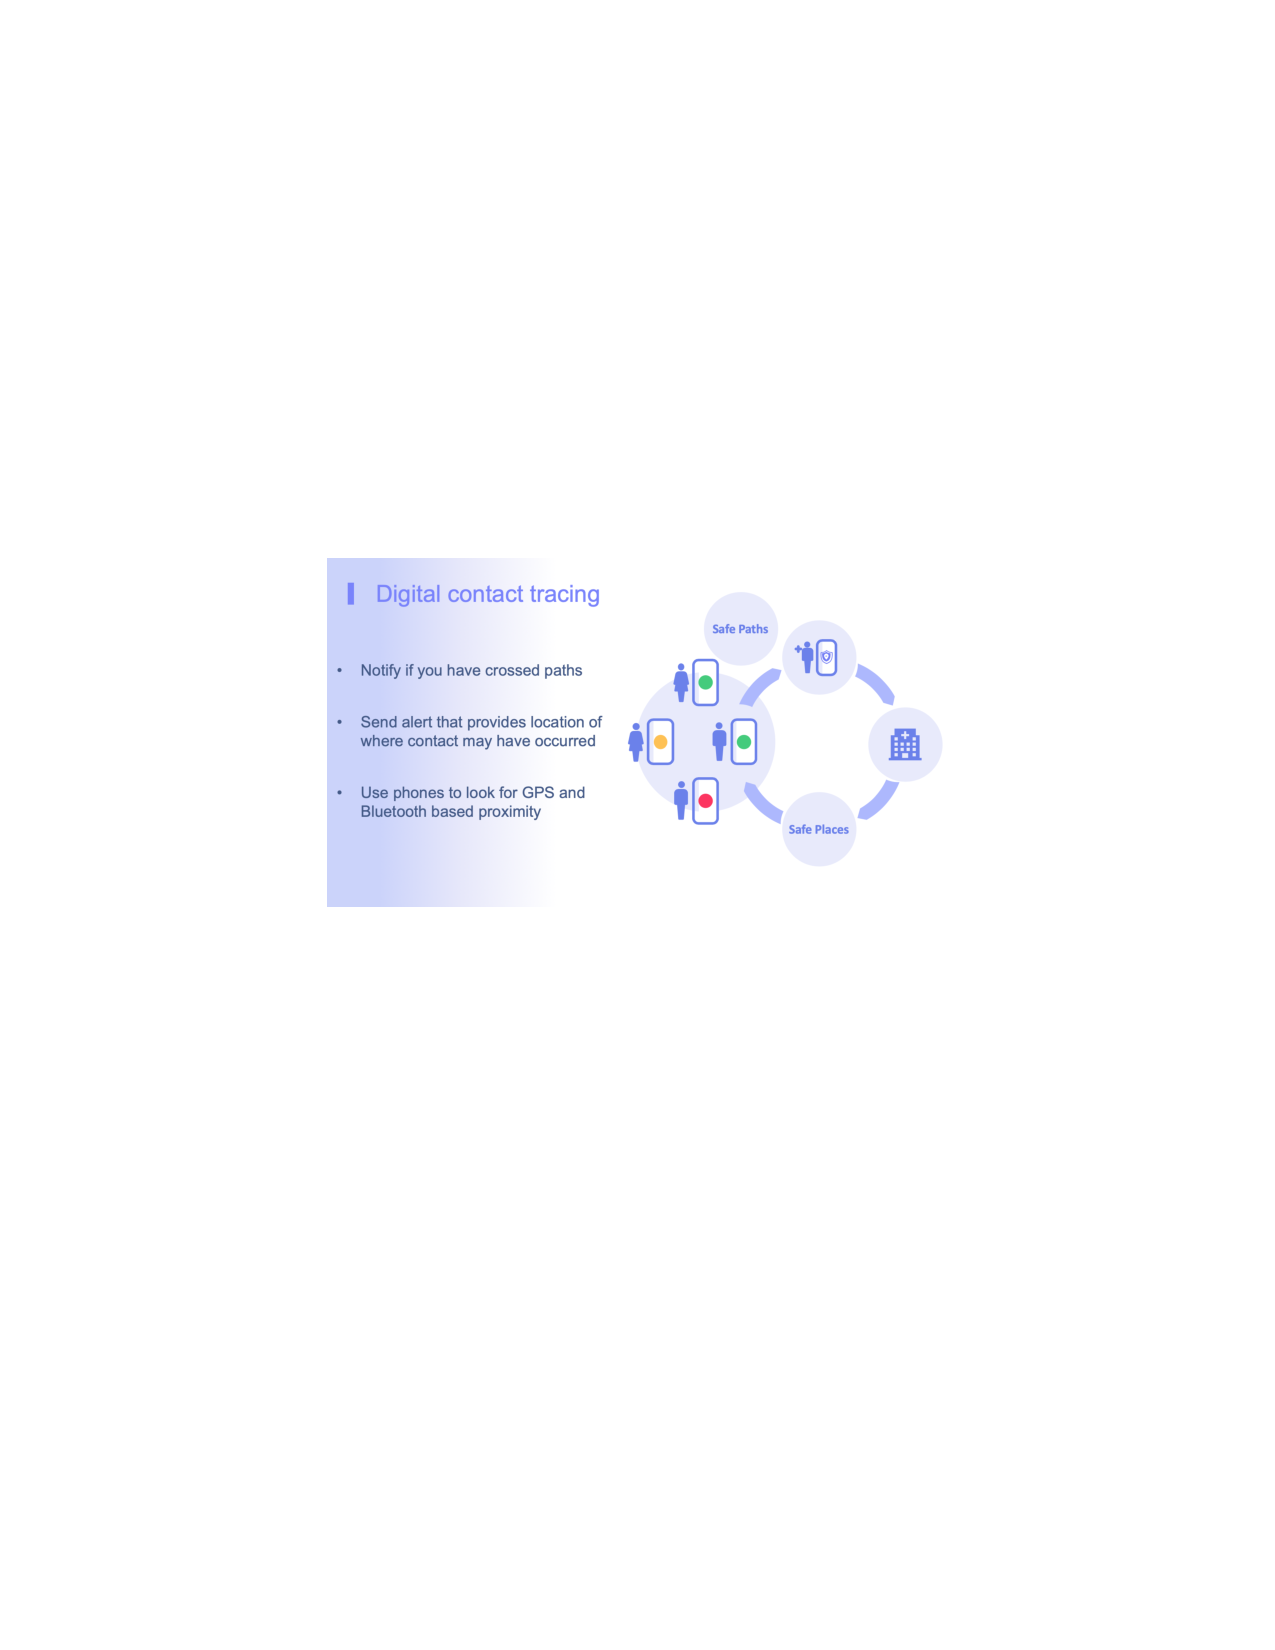
\includegraphics{main_fig}
% 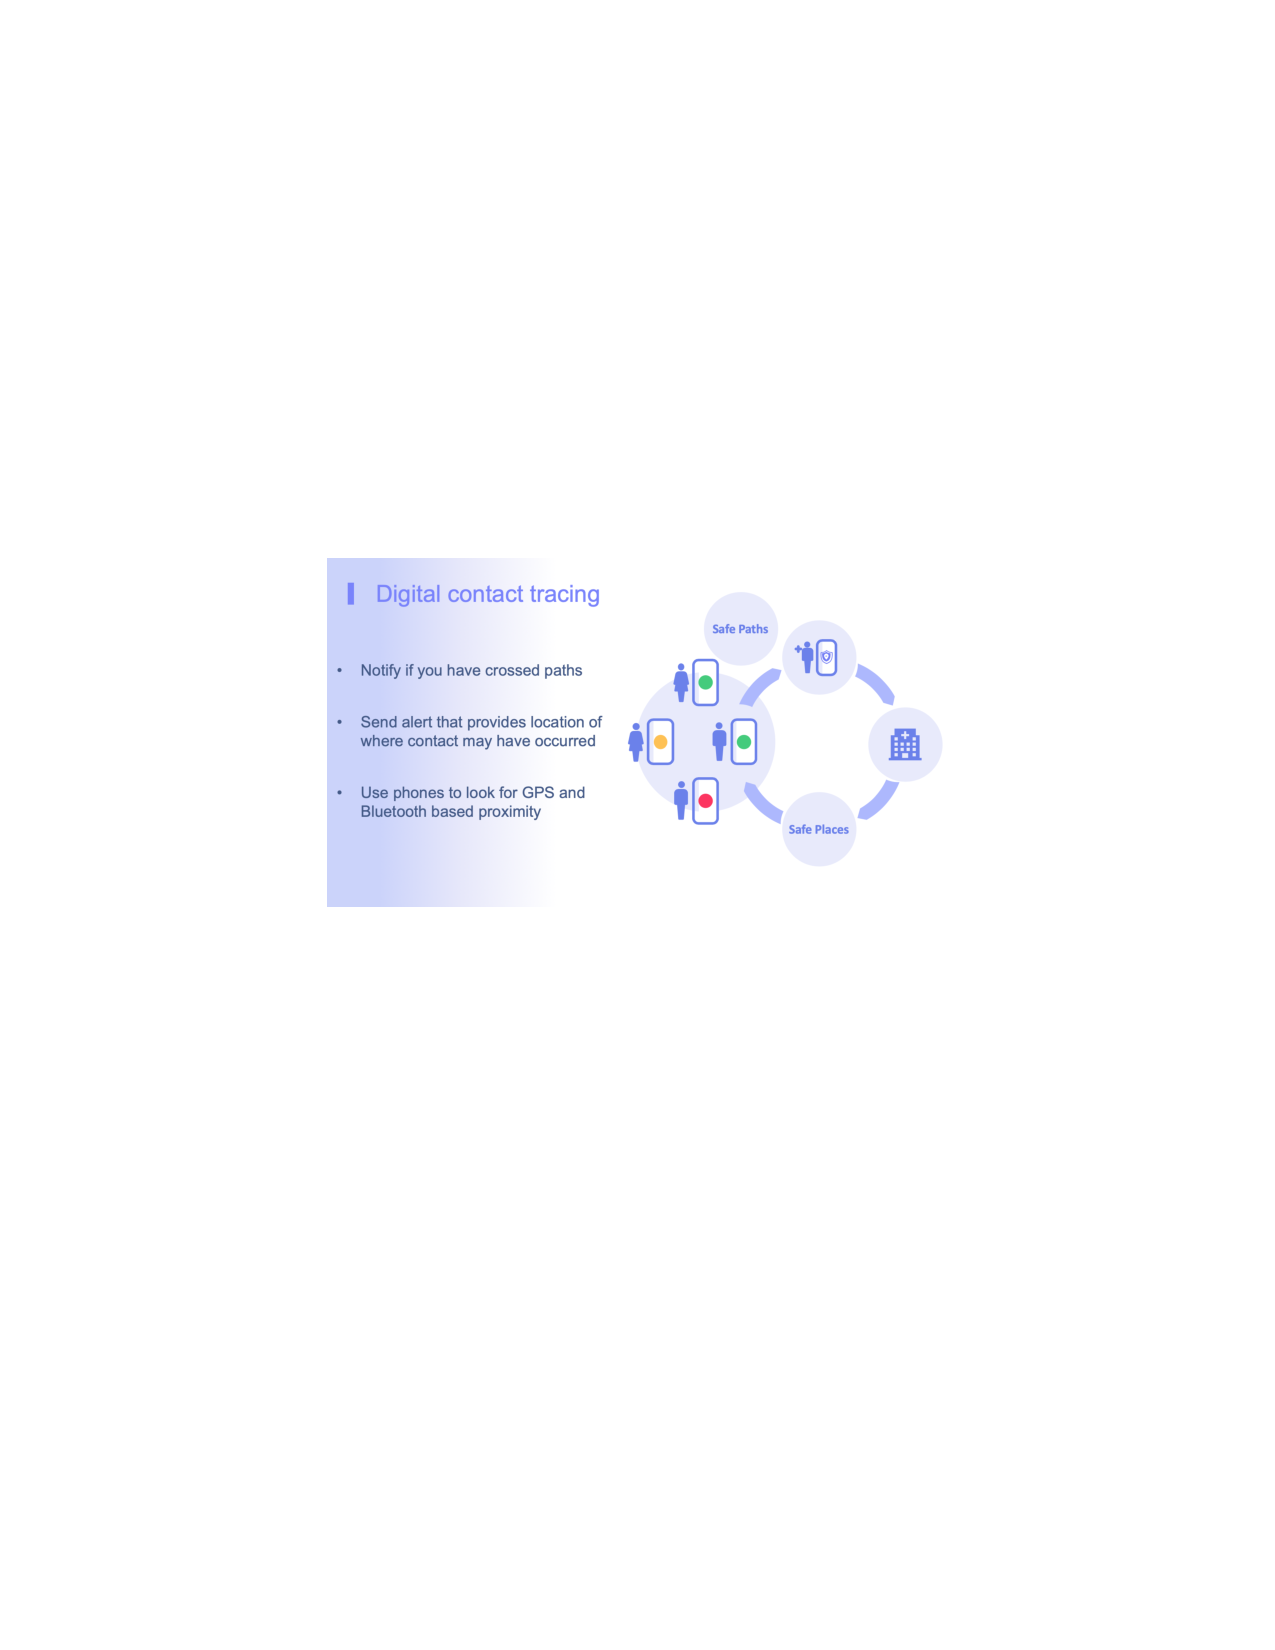
\includegraphics{main_fig}
\end{figure}


Contact tracing is just a tiny part of the public health interventions we need to build: for encounter memories, checking on loved ones or checking on co-workers you meet daily etc., health verification, sick leave certification and so on especially for restarting the economy. The tracing solution apps should be able to amplify the role of Public health officials. 

SafePaths is, above all, about building open standard end-to-end solutions for citizens and public health while maintaining privacy and scalability. We will continue to use the best tools, Bluetooth APIs included, to achieve this aim. In the early phases, the emphasis is on rapid iteration and deployment for solutions for epidemic tracking. In the later phases, the goal is building encrypted computational methods that can be useful in any future societal disruptions. In \cite{ramesh} Prof. Raskar's 2019 talk about creating an honest impartial broker to address challenges in a fragmented society.

We are already developing pilots in 30 jurisdictions across the world.  SafePaths is working closely with public health entities, and we plan to roll out apps and end-to-end solutions for each entity that makes use of  various technologies including the recent Apple/Google Bluetooth API. We are furthermore building interoperable protocols and standards, so that each of these jurisdictions can benefit and learn from each other.


\section{Safe Paths is Technology Agnostic}


We want to stress that Apple and Google are releasing Proximity AP but not a full contact tracing solution. The released APIs will give contact tracing tools such as Safe Paths the ability to work at a deeper level on phones, improving battery life, effectiveness and privacy. 


Here, it might be important to bring to light that while there are many contact tracing solutions that could be built on these APIs, there are issues of concern with relying on either one of the technologies alone - Bluetooth or GPS based solutions. In the case of Bluetooth, each phone (not just the infected person's phone) is emitting the Bluetooth ID every few seconds. So if an app is not transparent or open source, or runs afoul of other important privacy principles, there’s a great capacity for abuse, by listening in on the data of hundreds of millions of users as they broadcast IDs that change very slowly (15 mins). Smartphones can help reduce the spread of the virus but any network analysis could cause unacceptable intrusion to privacy and human rights. 


Conversely, the underlying data set for location data is much riskier than for Bluetooth data; that is, if you did share location data without privacy protection (either because of a poorly designed app, or by insufficient security protection), the results would be much more damaging than the release of BLE data (which is composed only of anonymous encrypted IDs).


In this vein, MIT SafePaths is in the process of building out both private tracing and a public health solution, part of which will utilize the new Google/Apple API, defined by two key elements:
\begin{enumerate}
\item open source software components
\item interoperable standards and backbone that work across GPS/BT/WiFi/Telecom
\end{enumerate}

We will be using either \emph{on-device} calculation or use \emph{encrypted trail match} with guarantees of privacy. Thus it avoids the ‘big brother’ surveillance state problem in certain countries where GPS matching solutions have been very effective but are draconian~\cite{ramesh2}. Such misinformation and distrust can cause civil unrest, especially in heterogeneous societies.


The vision at Safe Paths is to  enable a fusion of various technologies including GPS/Bluetooth/WiFi SSID to provide a more reliable approach, reduce false positives/negatives, provide context for believability and also provide aggregate dashboard view for public health officials. SafePaths is already delivering these technologies and will continue to build them in an open source way. Follow CovidSafePaths.org for a more technical discussion.



% \bibliographystyle{IEEEtran}
% \bibliography{submissions/safepaths/safepaths}
% % \bibliography{safepaths}



\begin{thebibliography}{1}
\providecommand{\url}[1]{#1}
\csname url@samestyle\endcsname
\providecommand{\newblock}{\relax}
\providecommand{\bibinfo}[2]{#2}
\providecommand{\BIBentrySTDinterwordspacing}{\spaceskip=0pt\relax}
\providecommand{\BIBentryALTinterwordstretchfactor}{4}
\providecommand{\BIBentryALTinterwordspacing}{\spaceskip=\fontdimen2\font plus
\BIBentryALTinterwordstretchfactor\fontdimen3\font minus
  \fontdimen4\font\relax}
\providecommand{\BIBforeignlanguage}[2]{{%
\expandafter\ifx\csname l@#1\endcsname\relax
\typeout{** WARNING: IEEEtran.bst: No hyphenation pattern has been}%
\typeout{** loaded for the language `#1'. Using the pattern for}%
\typeout{** the default language instead.}%
\else
\language=\csname l@#1\endcsname
\fi
#2}}
\providecommand{\BIBdecl}{\relax}
\BIBdecl

\bibitem{caseynewton}
\BIBentryALTinterwordspacing
C.~Newton, ``Why bluetooth apps are bad at discovering new cases of covid-19,''
  10 April 2020 (Accessed 30 May 2020). [Online]. Available:
  \url{https://web.archive.org/web/20200426200909/https://www.theverge.com/interface/2020/4/10/21215267/covid-19-contact-tracing-apps-bluetooth-coronavirus-flaws-public-health}
\BIBentrySTDinterwordspacing

\bibitem{ramesh}
\BIBentryALTinterwordspacing
R.~Raskar, ``God's eye view: Will global ai empower us or destroy us,''
  November 2019. [Online]. Available:
  \url{https://www.ted.com/talks/ramesh_raskar_god_s_eye_view_will_global_ai_empower_us_or_destroy_us}
\BIBentrySTDinterwordspacing

\bibitem{ramesh2}
R.~Raskar, I.~Schunemann, R.~Barbar, K.~Vilcans, J.~Gray, P.~Vepakomma,
  S.~Kapa, A.~Nuzzo, R.~Gupta, A.~Berke, D.~Greenwood, C.~Keegan, S.~Kanaparti,
  R.~Beaudry, D.~Stansbury, B.~B. Arcila, R.~Kanaparti, V.~Pamplona, F.~M.
  Benedetti, A.~Clough, R.~Das, K.~Jain, K.~Louisy, G.~Nadeau, V.~Pamplona,
  S.~Penrod, Y.~Rajaee, A.~Singh, G.~Storm, and J.~Werner, ``Apps gone rogue:
  Maintaining personal privacy in an epidemic,'' 2020.

\end{thebibliography}


\end{document}